
\documentclass{article}

\usepackage{tikz}
\usetikzlibrary{mindmap,trees}
\begin{document}
\pagestyle{empty}


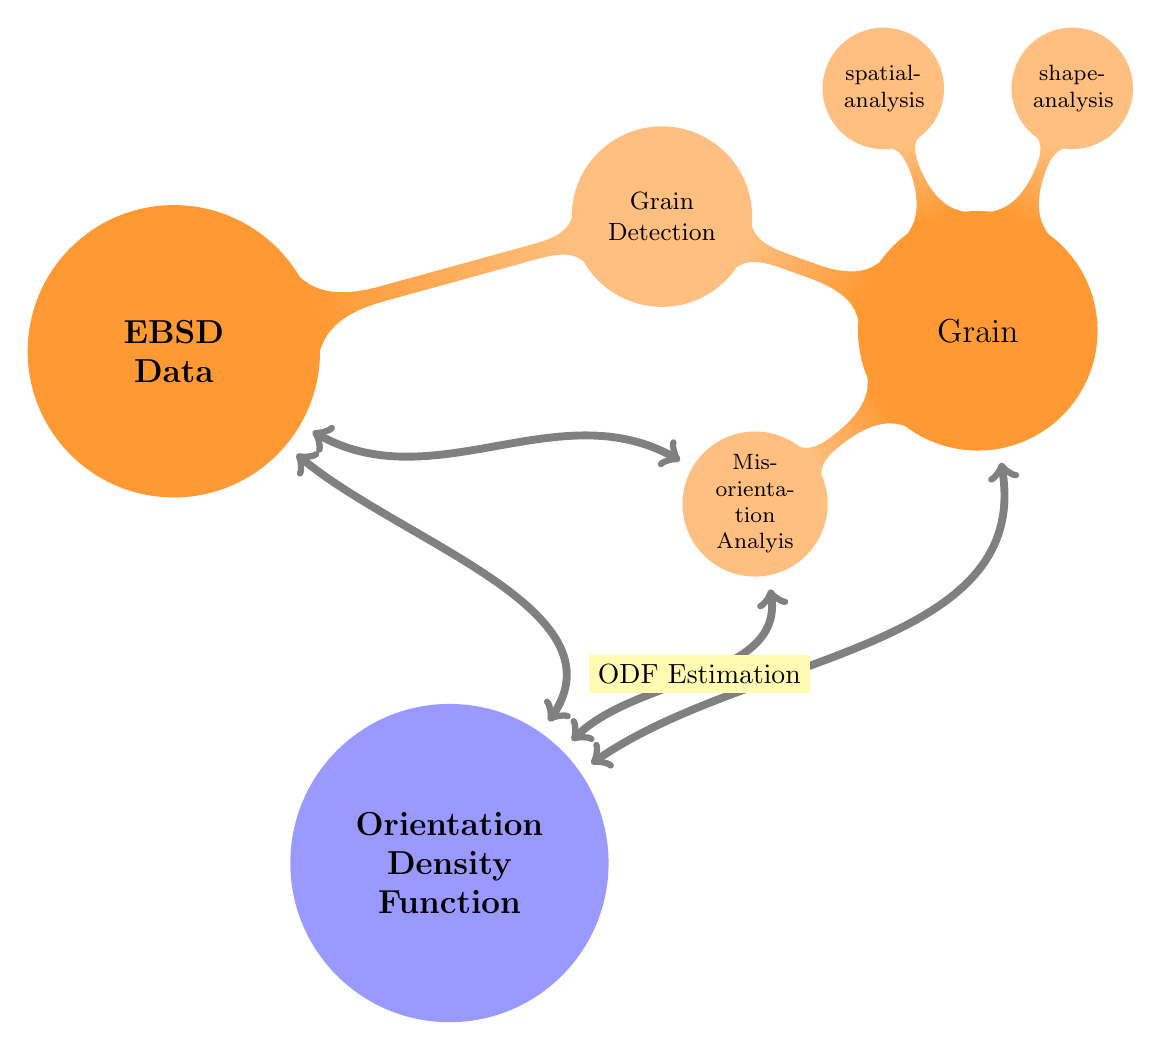
\begin{tikzpicture}[scale = 1]
  \definecolor{myblue}{HTML}{92dcec}
  \tikzstyle{every annotation}=[fill=white, font=\sf]

 \path[mindmap, concept color=orange!80!]
  node[concept,minimum size=3cm](ebsd) at (-3.5,6.5) {\bf EBSD \\Data} 
  child[grow = 20, concept color=orange!50] 
  { node(ebsd) [concept](ebsd2) at(0:1.5) { Grain \\ Detection} 
  		child[grow = -30, concept color=orange!80, minimum size = 3cm]  {  node [concept] (grain) at(0:1.5) {\large Grain} 
  			child[grow = 60, concept color=orange!50] 
  			{ node[concept, minimum size=1.5cm,font=\footnotesize](pf) at(0,1) {shape-analysis}}
  			child[grow = 120, concept color=orange!50] 
  			{ node[concept,minimum size=1.5cm,font=\footnotesize](pf) at(0,1) {spatial-analysis}}
  			child[grow = -150, concept color=orange!50] 
  			{ node[concept,minimum size=1.8cm,font=\footnotesize](miso) at(-0.75,-1) {Mis\-orienta\-tion Analyis}}}};
  

  \path[mindmap,concept color=blue!40!]
  node[concept](odf) {\bf Orientation Density Function};

	\draw [<->,concept connection] (ebsd) to[out=-30,in=150] (miso);
	
	\draw [<->,concept connection] (ebsd) to[out=-40,in=55] (odf); 
	\draw [<->,concept connection] (grain) to[out=-80,in=35] (odf);  
	\draw [<->,concept connection] (miso) to[out=-80,in=45]  node[fill=yellow!30] { ODF Estimation}(odf)  ;  

\end{tikzpicture}

\end{document}
%%% Local Variables: 
%%% mode: latex
%%% TeX-master: t
%%% End: 
